%%% CSE 4316 SRS - WORKED EXAMPLE (Autonomous Ground Robot)
%%% Structure follows ISO/IEC/IEEE 29148:2018. See ../../system requirements specification LaTeX/ for the blank template.
\documentclass[11pt,letterpaper]{article}
\usepackage[margin=1.0in]{geometry}
\usepackage[T1]{fontenc}
\usepackage[bitstream-charter]{mathdesign}
\usepackage[latin1]{inputenc}
\usepackage{amsmath}\usepackage{xcolor}\usepackage{cite}\usepackage{hyphenat}
\usepackage{graphicx}\usepackage{float}\usepackage{subfigure}\usepackage{sectsty}
\usepackage[compact]{titlesec}\usepackage[tablegrid]{vhistory}\usepackage{pbox}\usepackage{longtable}
\usepackage{tikz}\usetikzlibrary{positioning,arrows.meta,fit,backgrounds}
\allsectionsfont{\color{accentcolor}\scshape\selectfont}
\definecolor{accentcolor}{rgb}{0.0,0.0,0.5}
\tikzset{
  mod/.style={draw, rounded corners, fill=white, minimum height=8mm, minimum width=27mm, font=\footnotesize, align=center, inner sep=2pt},
  ext/.style={draw, dashed, rounded corners, fill=black!4, minimum height=8mm, minimum width=24mm, font=\footnotesize\itshape, align=center, inner sep=2pt},
  band/.style={draw=accentcolor!45, rounded corners, inner sep=3.5mm},
  llbl/.style={font=\small\bfseries, text=accentcolor, align=left},
  flow/.style={-{Latex[length=2mm]}, thick, draw=accentcolor!80},
  fl/.style={font=\scriptsize, fill=white, inner sep=1pt},
}
\newcommand{\teamname}{Team Trailblazer}
\newcommand{\productname}{TerraScout Autonomous Ground Rover}
\newcommand{\coursename}{CSE 4316: Senior Design I}
\newcommand{\semester}{Fall 2026}
\newcommand{\docname}{System Requirements Specification}
\newcommand{\department}{Department of Computer Science \& Engineering}
\newcommand{\university}{The University of Texas at Arlington}
\newcommand{\authors}{Alan Turing \\ Grace Hopper \\ John Von Neumann \\ Ada Lovelace \\ Charles Babbage}
\usepackage{fancyhdr}\pagestyle{fancy}\usepackage{lastpage}
\lhead{}\chead{}\rhead{}\lfoot{\footnotesize \teamname \ - \semester}\cfoot{}
\rfoot{\footnotesize page \thepage\ of \pageref{LastPage}}
\renewcommand{\headrulewidth}{0.0pt}\renewcommand{\footrulewidth}{0.4pt}
\usepackage[runin]{abstract}\abslabeldelim{\quad}\setlength{\abstitleskip}{-10pt}
\renewcommand{\abstractname}{}\renewcommand{\abstracttextfont}{\color{accentcolor} \small \slshape}

% requirement attribute helper
\newcommand{\req}[7]{%
  \subsubsection*{Description} #1
  \subsubsection*{Rationale} #2
  \subsubsection*{Source} #3
  \subsubsection*{Priority} #4
  \subsubsection*{Verification Method} #5
  \subsubsection*{Constraints} #6
  \subsubsection*{Applicable Standards} #7
}

\begin{document}
{\centering \huge \color{accentcolor} \sc \textbf{\department \\ \university} \par}
\vspace{1 in}
{\centering \huge \color{accentcolor} \sc \textbf{\docname \\ \coursename \\ \semester} \par}
\vspace{0.5 in}
\begin{figure}[h!]\centering
\includegraphics[width=0.60\textwidth]{images/test_image}\end{figure}
\vspace{0.5 in}
{\centering \huge \color{accentcolor} \sc \textbf{\teamname \\ \productname} \par}
\vspace{0.5 in}
{\centering \large \sc \textbf{\authors} \par}
\newpage

\begin{versionhistory}
  \vhEntry{0.1}{10.01.2026}{GH}{document creation}
  \vhEntry{0.2}{10.08.2026}{AL|JVN}{complete draft}
  \vhEntry{1.0}{10.20.2026}{AT|GH|CB}{official release}
\end{versionhistory}
\newpage
\setcounter{tocdepth}{2}\tableofcontents
\newpage

\section{Introduction}
This SRS specifies the requirements for \productname, an autonomous ground rover
for photovoltaic (PV) field inspection. It follows the SRS information item of
ISO/IEC/IEEE 29148:2018 \cite{ISO29148}.

\subsection{Purpose}
This document is the agreed requirements baseline between Team Trailblazer and the
sponsor. Requirements herein may not be changed without the sponsor's agreement.

\subsection{Scope}
The system shall autonomously patrol drivable lanes of a PV field along
operator-defined GPS waypoints, capture RGB and thermal imagery of panels, detect
likely faults on-board, produce a GPS-tagged inspection report, and return to a
charging dock autonomously. Off-board analytics dashboards and cloud storage are
out of scope for the prototype.

\subsection{Product Overview}
\subsubsection{Product Perspective}
The rover is a self-contained mobile system that interoperates with two external
elements: an operator ground-station laptop (over Wi-Fi) and a passive charging
dock. See Figure~\ref{fig:ctx}.
\begin{figure}[h!]\centering\resizebox{0.68\textwidth}{!}{%
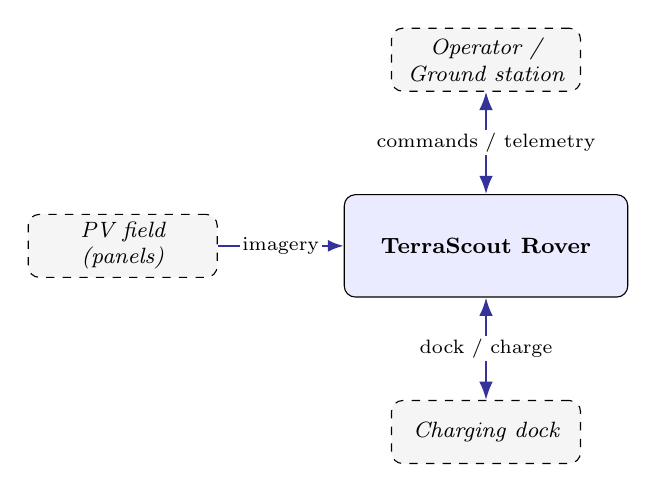
\begin{tikzpicture}
\node[mod, minimum width=36mm, minimum height=13mm, fill=blue!8] (sys) {\textbf{TerraScout Rover}};
\node[ext, above=13mm of sys] (op) {Operator /\\Ground station};
\node[ext, left=16mm of sys] (pv) {PV field\\(panels)};
\node[ext, below=13mm of sys] (dock) {Charging dock};
\draw[{Latex}-{Latex}, thick, draw=accentcolor!80] (sys) -- (op) node[fl,pos=0.5]{commands / telemetry};
\draw[flow] (pv) -- (sys) node[fl,pos=0.5]{imagery};
\draw[{Latex}-{Latex}, thick, draw=accentcolor!80] (sys) -- (dock) node[fl,pos=0.5]{dock / charge};
\end{tikzpicture}}
\caption{System context: rover, ground station, and charging dock}\label{fig:ctx}\end{figure}
\subsubsection{Product Functions}
Tele-operated and autonomous driving; waypoint navigation with obstacle avoidance;
RGB/thermal capture; on-board fault detection; GPS-tagged report generation;
autonomous dock and recharge; ground-station monitoring and control.
\subsubsection{User Characteristics}
The primary user is a field O\&M technician: comfortable with tablets/laptops, not
a roboticist, operating outdoors in PPE. A secondary maintainer role (team/engineer)
services hardware and software.
\subsubsection{Assumptions \& Dependencies}
Drivable lanes $\leq$10\% grade; RTK-GPS correction available; private Wi-Fi
between rover and ground station; daylight, dry-weather operation.

\subsection{Definitions, Acronyms, and Abbreviations}
\begin{table}[H]\begin{center}
\begin{tabular}{ | p{3cm} | p{10cm} |}\hline
\textbf{Term} & \textbf{Definition} \\ \hline
PV & Photovoltaic (solar) panel \\ \hline
Hotspot & Localized thermal anomaly indicating a likely panel fault \\ \hline
RTK & Real-Time Kinematic GPS correction (centimeter-level positioning) \\ \hline
Waypoint & An operator-defined GPS coordinate on the patrol route \\ \hline
Ground station & Operator laptop running the control/monitoring web page \\ \hline
\end{tabular}\end{center}\end{table}
\newpage

\section{Requirements Engineering Approach}
Requirements use identifiers \texttt{[TYPE]-[NN]} (EI, FR, US, PE, PK, SA, SE, MS,
QA) and carry the ISO/IEC/IEEE 29148 attribute set: Description, Rationale, Source,
Priority (Critical/High/Moderate/Low/Future), Verification Method
(Inspection/Analysis/Demonstration/Test), Constraints, and Applicable Standards.
Each requirement is written to be singular, unambiguous, and verifiable.
\newpage

\section{External Interface Requirements}
\subsection{EI-01: Ground-station control link}
\req{The rover shall expose a WebSocket control/telemetry link over TLS on the
private Wi-Fi network, accepting start/stop/return commands and streaming pose,
battery, and status at $\geq$2\,Hz.}
{The operator must command runs and observe live status from the ground station.}
{Sponsor scoping interview; team.}
{Critical}
{Test --- exercise each command and measure telemetry rate.}
{Wi-Fi range limits operating radius; link loss triggers safe-stop (see FR-05).}
{IETF RFC 6455 (WebSocket), RFC 8446 (TLS 1.3).}
\subsection{EI-02: Charging dock interface}
\req{The rover shall mate with the charging dock and draw charge current through a
polarized contact pair when docked.}
{Enables autonomous recharge without operator handling.}
{Team.}
{High}
{Demonstration --- rover docks and charging begins.}
{Contact alignment tolerance $\pm$20\,mm from approach heading.}
{UL~2089 (vehicle battery charging), as guidance.}

\section{Functional Requirements}
\subsection{FR-01: Waypoint patrol}
\req{Given an ordered list of GPS waypoints, the rover shall drive to each in
sequence within a 0.5\,m cross-track tolerance and signal completion.}
{Consistent, repeatable coverage of PV rows is the core inspection function.}
{Sponsor.}
{Critical}
{Test --- run a surveyed course; measure cross-track error.}
{Requires RTK correction; degraded to 2\,m tolerance without RTK.}
{None specific.}
\subsection{FR-02: Imagery capture}
\req{At each panel-row segment the rover shall capture time- and GPS-stamped RGB
and thermal frames covering the adjacent panel faces.}
{Imagery is the evidence from which faults are detected and reported.}
{Sponsor.}
{Critical}
{Test --- verify frames exist, are stamped, and cover the panels.}
{Thermal resolution limited by loaned camera.}
{EXIF GPS tagging.}
\subsection{FR-03: On-board fault detection}
\req{The rover shall classify each captured panel region as \textit{nominal} or
\textit{suspected fault} (hotspot/soiling/crack) and record the location.}
{Detecting faults on-board avoids shipping all imagery for manual review.}
{Sponsor; team.}
{High}
{Test --- run against a labeled validation set; report precision/recall (see PE-03).}
{Model runs within the compute budget of the on-board module.}
{None specific.}
\subsection{FR-04: Inspection report}
\req{At end of run the rover shall produce a report listing each suspected fault
with GPS coordinate, timestamp, class, and a reference image, downloadable from the
ground station.}
{The report is the deliverable the O\&M team acts on.}
{Sponsor.}
{Critical}
{Demonstration --- generate and download a report after a run.}
{Report format agreed with sponsor (CSV + image bundle).}
{None specific.}
\subsection{FR-05: Safe-stop \& autonomous return}
\req{On obstacle, low battery ($\leq$20\%), or control-link loss $>$10\,s, the rover
shall halt safely and, when able, navigate autonomously to the charging dock.}
{Protects the platform and surroundings and enables unattended operation.}
{Team; safety review.}
{Critical}
{Test --- inject each trigger and observe safe-stop/return.}
{Return requires a known dock waypoint and sufficient reserve charge.}
{None specific.}

\section{Usability Requirements}
\subsection{US-01: One-page operation}
\req{A trained technician shall start a patrol, monitor it, and download the report
using a single ground-station web page, completing setup in under 3 minutes in
$\geq$8 of 10 trials.}
{Field staff are not roboticists; operation must be simple.}
{Sponsor.}
{High}
{Test --- moderated usability trials.}
{Readable outdoors in daylight on a laptop screen.}
{WCAG 2.2 AA for the web page.}

\section{Performance Requirements}
\subsection{PE-01: Patrol throughput}
\req{The rover shall inspect at least 200 panels per hour under nominal conditions.}
{Determines how much of a site can be covered per charge/day.}
{Sponsor.}
{High}{Test --- timed field run.}{Bounded by drive speed and capture dwell time.}{None.}
\subsection{PE-02: Endurance}
\req{The rover shall operate for at least 45 minutes of continuous patrol on one charge.}
{Sets usable run length between docks.}
{Team.}{High}{Test --- discharge run to 20\%.}{Battery capacity/weight budget.}{None.}
\subsection{PE-03: Detection quality}
\req{On-board fault detection shall achieve $\geq$0.80 recall and $\geq$0.70
precision on the sponsor-provided validation set.}
{Missed faults defeat the purpose; excessive false alarms waste truck-rolls.}
{Sponsor; team.}
{High}{Analysis --- evaluate against labeled set.}{Limited by training data volume.}{None.}

\section{Packaging \& Deployment Requirements}
\subsection{PK-01: Field-deployable unit}
\req{The rover shall be delivered as a single assembled unit with the charging dock
and a USB drive containing the ground-station application and operator manual.}
{The sponsor receives a ready-to-run system, not a kit.}
{Sponsor.}{Moderate}{Inspection.}{Two-person liftable ($<$25\,kg).}{None.}

\section{Safety Requirements}
\subsection{SA-01: Emergency stop}
\req{The rover shall provide a physical, latching emergency-stop that removes power
from the drive motors when pressed.}
{Immediate manual means to stop motion is a baseline safety control.}
{Safety review; lab policy.}
{Critical}{Demonstration --- press E-stop under motion; motors de-energize.}
{E-stop reachable on the chassis top surface.}{ISO 13850 (emergency stop).}
\subsection{SA-02: Laboratory LOTO}
\req{Fabrication equipment shall be used per OSHA lockout/tagout procedures; only
the instructor or TAs may remove a lock.}
{Prevents injury during fabrication.}
{CSE Senior Design laboratory policy.}
{Critical}{Inspection.}{Availability of instructor/TA to remove locks.}
{OSHA 29 CFR 1910.147.}

\section{Security \& Privacy Requirements}
\subsection{SE-01: Encrypted control link}
\req{All ground-station$\leftrightarrow$rover traffic shall be encrypted with TLS
1.3; unauthenticated command sessions shall be refused.}
{Prevents hijacking of a moving robot and tampering with reports.}
{Team; security review.}
{Critical}{Test --- protocol scan; attempt unauthenticated command.}
{Pre-shared credential provisioned at setup.}
{IETF RFC 8446 (TLS 1.3).}
\subsection{SE-02: Site imagery handling}
\req{Captured site imagery shall remain on the rover/ground station and shall not
be transmitted off the private network without sponsor approval.}
{Solar-site imagery may be sensitive to the sponsor.}
{Sponsor.}{High}{Inspection --- data-flow review.}{No cloud egress in prototype.}{None.}

\section{Maintenance \& Support Requirements}
\subsection{MS-01: Diagnosable faults}
\req{The rover shall log each subsystem fault with a timestamp and error code
retrievable from the ground station without a debugger.}
{Field maintainers must localize failures quickly.}
{Team.}{Moderate}{Demonstration.}{Log storage sized for a day of operation.}{None.}

\section{Other Quality Attributes}
\subsection{QA-01: Modular perception}
\req{The fault-detection model shall be replaceable without changes to the
navigation or platform software.}
{Allows the detector to improve independently as more data is collected.}
{Team.}{Moderate}{Inspection --- interface review.}{Defined model interface.}
{ISO/IEC 25010:2023 (modularity) \cite{ISO25010}.}

\section{Verification \& Traceability}
\begin{longtable}{ | p{1.4cm} | p{6.6cm} | p{1.4cm} | p{3cm} |}\hline
\textbf{Req ID} & \textbf{Requirement (abbrev.)} & \textbf{Method} & \textbf{Acceptance} \\ \hline\endhead
FR-01 & Waypoint patrol within 0.5\,m & T & cross-track $\leq$0.5\,m \\ \hline
FR-03 & On-board fault detection & T & meets PE-03 \\ \hline
FR-05 & Safe-stop \& return & T & all triggers handled \\ \hline
PE-01 & $\geq$200 panels/hour & T & measured $\geq$200 \\ \hline
PE-03 & Detection quality & A & recall $\geq$0.80, prec.\ $\geq$0.70 \\ \hline
SE-01 & TLS 1.3 control link & T & scan shows TLS1.3; unauth refused \\ \hline
\end{longtable}
Full requirement-to-design-to-test traceability is maintained in the team's shared
matrix and extended in the ADS, DDS, and Test Plan.

\section{Future Items}
\subsection{FI-01: Cloud analytics dashboard}
\req{A hosted dashboard aggregating fault trends across runs and sites.}
{Adds fleet-level insight but exceeds prototype budget/time.}
{Sponsor.}{Future}{Test (if implemented).}{Requires cloud hosting and data egress.}{None.}

\bibliographystyle{reference/IEEEtran_custom}
\bibliography{reference/refs}{}
\end{document}
